\documentclass[runningheads]{llncs}
\usepackage[T1]{fontenc}
\usepackage{graphicx}
\usepackage{amsmath,amssymb}
\usepackage{booktabs}
\usepackage{xcolor}
\usepackage[hidelinks]{hyperref}
\graphicspath{{figures/}}

% Same result macros as the main paper: every reported number is regenerated from the experiment output.
\newcommand{\na}{\textcolor{gray}{--}}
% Auto-generated by scripts/fill_paper_results.py. Do not edit by hand.
\providecommand{\na}{--}
\newcommand{\ablIouFull}{0.41}
\newcommand{\ablIouLm}{0.39}
\newcommand{\ablIouSeg}{0.30}
\newcommand{\ablIouTc}{0.42}
\newcommand{\ablLocFull}{27.1}
\newcommand{\ablLocLm}{28.6}
\newcommand{\ablLocSeg}{13.7}
\newcommand{\ablLocTc}{26.3}
\newcommand{\ablWFull}{0.115}
\newcommand{\ablWLm}{0.111}
\newcommand{\ablWSeg}{0.129}
\newcommand{\ablWTc}{0.106}
\newcommand{\diceCanon}{0.50}
\newcommand{\diceGroup}{0.66}
\newcommand{\fidCUT}{235.6}
\newcommand{\fidCUTCurvi}{72.3}
\newcommand{\fidCyc}{\textbf{192.2}}
\newcommand{\fidCycCurvi}{\textbf{67.9}}
\newcommand{\fidPhys}{315.3}
\newcommand{\fidPhysCurvi}{212.9}
\newcommand{\fidSCyc}{199.7}
\newcommand{\fidSCycCurvi}{104.2}
\newcommand{\fidSono}{294.7}
\newcommand{\fidSonoCurvi}{191.1}
\newcommand{\inReg}{0.065}
\newcommand{\iouCUT}{0.17}
\newcommand{\iouCyc}{0.11}
\newcommand{\iouPhys}{\textbf{1.00}}
\newcommand{\iouSCyc}{0.13}
\newcommand{\iouSono}{0.41}
\newcommand{\iouSonoCurvi}{0.54}
\newcommand{\kidCUT}{245.9}
\newcommand{\kidCUTCurvi}{55.9}
\newcommand{\kidCyc}{203.1}
\newcommand{\kidCycCurvi}{\textbf{55.6}}
\newcommand{\kidPhys}{294.3}
\newcommand{\kidPhysCurvi}{265.4}
\newcommand{\kidSCyc}{\textbf{196.9}}
\newcommand{\kidSCycCurvi}{84.2}
\newcommand{\kidSono}{306.5}
\newcommand{\kidSonoCurvi}{232.6}
\newcommand{\liverDice}{0.93}
\newcommand{\locCUT}{0.0}
\newcommand{\locCyc}{0.0}
\newcommand{\locPhys}{0.0}
\newcommand{\locSCyc}{0.0}
\newcommand{\locSono}{\textbf{26.3}}
\newcommand{\locSonoCurvi}{18.6}
\newcommand{\locality}{26}
\newcommand{\lungDice}{0.90}
\newcommand{\outReg}{0.005}
\newcommand{\softCanon}{0.35}
\newcommand{\softGroup}{0.75}
\newcommand{\tstrCUT}{0.031}
\newcommand{\tstrCyc}{0.032}
\newcommand{\tstrPhys}{0.049}
\newcommand{\tstrPhysCurvi}{0.097}
\newcommand{\tstrPhysCurviSd}{0.006}
\newcommand{\tstrPhysTent}{0.106}
\newcommand{\tstrPhysTentSd}{0.006}
\newcommand{\tstrSCyc}{0.026}
\newcommand{\tstrSono}{0.025}
\newcommand{\tstrSonoCurvi}{0.099}
\newcommand{\tstrSonoCurviSd}{0.011}
\newcommand{\tstrSonoTent}{0.124}
\newcommand{\tstrSonoTentSd}{0.007}
\newcommand{\ttaSeeds}{5}
\newcommand{\vesselDice}{0.72}
\newcommand{\wCUT}{0.246}
\newcommand{\wCyc}{0.266}
\newcommand{\wPhys}{0.064}
\newcommand{\wPhysCurvi}{0.056}
\newcommand{\wSCyc}{0.223}
\newcommand{\wSono}{\textbf{0.119}}
\newcommand{\wSonoCurvi}{0.115}

% Per-tissue in-the-loop results (organ-conditioned liver acquisition).
% Recognition = a REAL-trained organ recognizer J on held-out simulator content, crop-domain-matched
%   J, 3 seeds (scripts/premise/, aggregate.py). RL = organ-conditioned liver acquisition, 3 seeds,
%   held-out patients (scripts/train_organ_rl.py, agg_organ_rl.py). See docs/PREMISE_CHECK_RESULT.md.
\newcommand{\recSono}{0.48}
\newcommand{\recCut}{0.21}
\newcommand{\recCyc}{0.14}
\newcommand{\recPhys}{0.27}
\newcommand{\recCeil}{0.51}
\newcommand{\rlSono}{0.152}
\newcommand{\rlSonoSd}{0.004}
\newcommand{\rlCut}{0.144}
\newcommand{\rlCyc}{0.142}
\newcommand{\rlPhys}{0.142}
\newcommand{\rlStart}{0.11}
\newcommand{\rewSono}{0.32}
\newcommand{\rewPhys}{0.20}
\newcommand{\rewCut}{0.18}
\newcommand{\rewCyc}{0.16}
\newcommand{\rlSeeds}{3}


% Number floats as S1, S2, ... so they match the "supplementary Table S1 / Fig. S1" references in the paper.
\renewcommand{\thetable}{S\arabic{table}}
\renewcommand{\thefigure}{S\arabic{figure}}

\begin{document}

\title{SonoSPADE: Supplementary Material}
\titlerunning{SonoSPADE: Supplementary Material}
\author{Thanapong Intharah\inst{1} \and Zhichao Gao\inst{2} \and Hao Dong\inst{2}}
\authorrunning{T. Intharah et al.}
\institute{Visual Intelligence Laboratory, Khon Kaen University, Khon Kaen, Thailand\\
\email{thanapong.intharah@gmail.com}
\and School of Computer Science, Peking University, Beijing, China}
\maketitle

\noindent This supplement collects the whole-frame FID/KID scores (Table~\ref{tab:fidkid}), the
training-term ablation (Table~\ref{tab:abl}), the per-tissue label-swap locality breakdown
(Table~\ref{tab:locality_pertissue}), and the per-tissue qualitative result (Fig.~\ref{fig:qual})
referenced in the main paper. All numbers are generated from the same result files as the main tables.

\begin{table}[h]
\centering
\caption{Whole-frame FID/KID ($\times 10^{3}$) against the real pool (InceptionV3), lower better.
SonoSPADE is not competitive by design, because these metrics reward the global recolor it does not
perform. The bottom block re-runs in the sector geometry, which improves all absolute scores but not the
ranking.}
\label{tab:fidkid}
\begin{tabular}{lcc}
\toprule
Method & FID $\downarrow$ & KID $\times 10^{3}$ $\downarrow$\\
\midrule
Raw physics            & \fidPhys & \kidPhys\\
CycleGAN               & \fidCyc  & \kidCyc\\
CUT                    & \fidCUT  & \kidCUT\\
S-CycleGAN (reimpl.)   & \fidSCyc & \kidSCyc\\
SonoSPADE              & \fidSono & \kidSono\\
\midrule
Raw physics-curvi      & \fidPhysCurvi  & \kidPhysCurvi\\
CycleGAN-curvi         & \fidCycCurvi   & \kidCycCurvi\\
CUT-curvi              & \fidCUTCurvi   & \kidCUTCurvi\\
S-CycleGAN-curvi       & \fidSCycCurvi  & \kidSCycCurvi\\
SonoSPADE-curvi        & \fidSonoCurvi  & \kidSonoCurvi\\
\bottomrule
\end{tabular}
\end{table}

\begin{table}[h]
\centering
\caption{Ablation (one term off per row, each retrained at a fixed budget). Removing the frozen $S_{US}$
seg-consistency term roughly halves locality and degrades structure, the largest single effect. This is
the full version of the ablation summarized in Sec.~4.5 of the main paper.}
\label{tab:abl}
\begin{tabular}{lccc}
\toprule
Variant & Edge IoU $\uparrow$ & Organ $W_1$ $\downarrow$ & Locality $\uparrow$\\
\midrule
Full SonoSPADE          & \ablIouFull & \ablWFull & \ablLocFull\\
$-$ $S_{US}$ consistency & \ablIouSeg  & \ablWSeg  & \ablLocSeg\\
$-$ OASIS LabelMix       & \ablIouLm   & \ablWLm   & \ablLocLm\\
$-$ temporal consistency & \ablIouTc   & \ablWTc   & \ablLocTc\\
\bottomrule
\end{tabular}
\end{table}

\begin{table}[h]
\centering
\caption{Per-tissue label-swap locality on the physics/label content frames (higher means the texture
change is more localized to the relabeled region). Liver is the reference tissue and is excluded; spleen
and muscle rarely reach the $200$-pixel minimum in the content frames and are omitted. The values are the
measured per-class means behind the main-paper locality of $26.3$ (they average to it). Per-frame standard
deviations can be added with \texttt{scripts/eval\_locality\_std.py}.}
\label{tab:locality_pertissue}
\begin{tabular}{lc}
\toprule
Tissue & Label-swap locality $\uparrow$\\
\midrule
Gallbladder            & $22.8$\\
Vessel                 & $18.7$\\
Kidney                 & $30.2$\\
GI tract               & $40.3$\\
Pancreas               & $28.8$\\
Fat                    & $10.4$\\
Bone                   & $60.7$\\
Lung                   & $13.0$\\
Soft tissue            & $11.5$\\
\midrule
All tissues (mean)     & $26.3$\\
Label-free translators & $0$ (by construction)\\
\bottomrule
\end{tabular}
\end{table}

\begin{figure}[h]
\centering
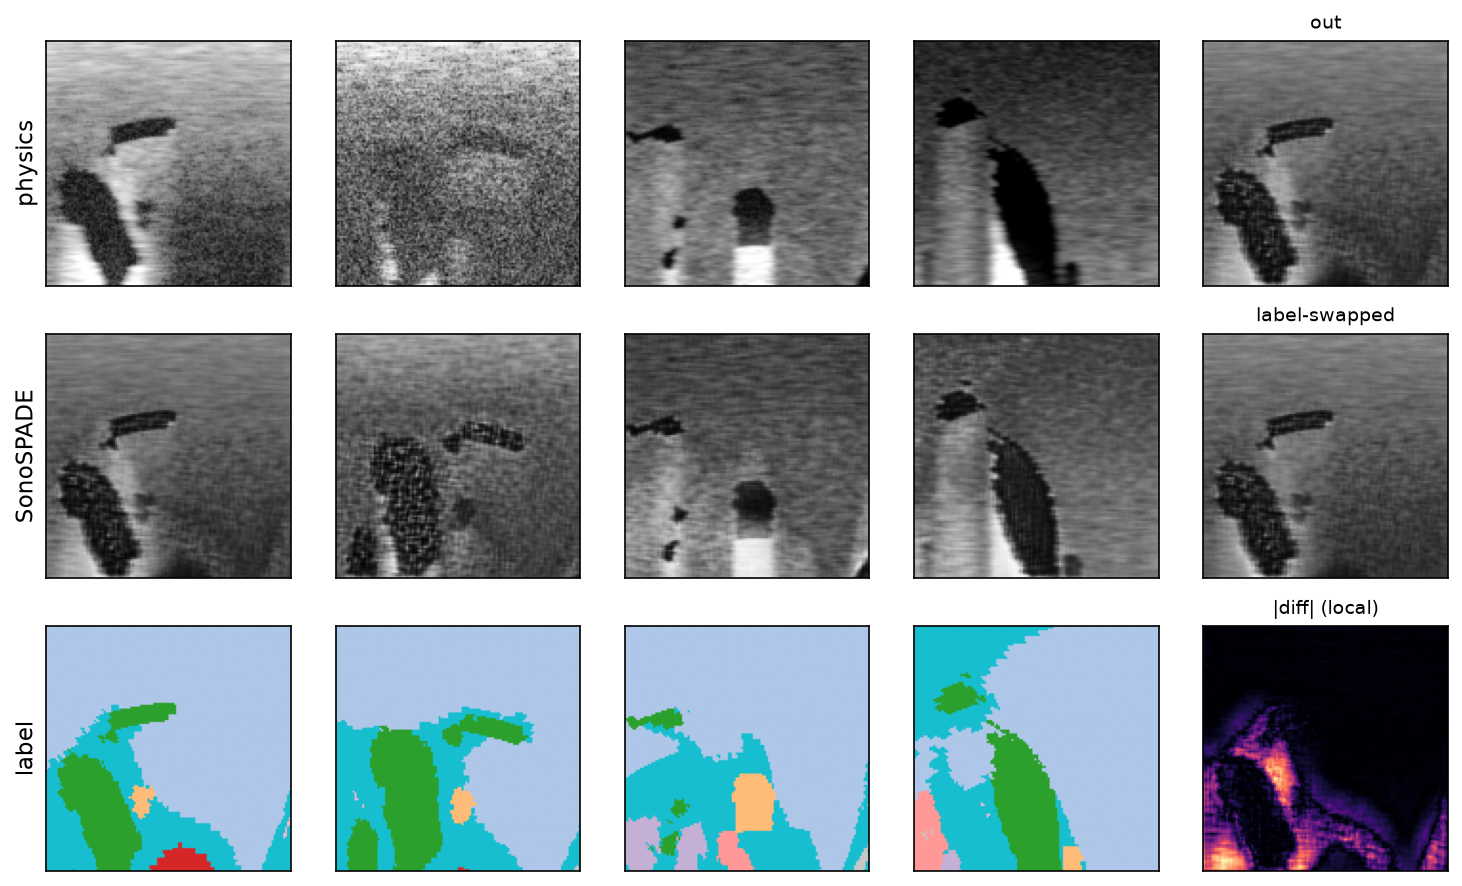
\includegraphics[width=0.85\linewidth]{qualitative.png}
\caption{Per-tissue qualitative result (Sec.~4.2 of the main paper). The rows are the physics render, the
SonoSPADE output, and the tissue label. Each tissue gets its own speckle, and relabeling a region changes
its texture locally (last column): the swapped region's texture changes while the rest of the frame stays
put, which is what the label-swap locality metric measures.}
\label{fig:qual}
\end{figure}

\end{document}
